\chapter{CNN Features Hashing}

\label{chapter:CNNFeaturesHashing}

% ----------------

% ---------------- Section: Introduction ----------------
\section{Introduction}
In a previous chapter \ref{chapter:HashingDimensionalityReduction}, we advocate the use of small binary codes and hashing for nearest neighbor search. In this chapter, we present a new approach for hashing into binary codes inspired from LSH with random projection and Minimal Loss Hashing, which are detailed in \ref{chapter:HashingDimensionalityReduction}.
	
Our approach is based on the same space partitioning as LSH with random projection and on the same cost function as Minimal Loss Hashing, it is therefore a supervised learning approach. The space is partitioned with a set of hyperplanes, each of them being responsible for the value of one bit in the binary code. If a point is on one side of a hyperplane, the associated bit takes a value of 1 and if the point is on the other side, the bit takes a value of 0. The difference between Minimal Loss Hashing and our approach is the optimization method. Minimal Loss Hashing builds a convex-concave upper bound on the loss function and a stochastic gradient-based method is used to minimize the bound function. On our side, we optimize the cost function in a continuous space. During the training, instead of binary codes, our algorithm generates $q$-dimensional vectors whose elements are in $[0, 1]$. Because codes are continuous, optimization is easier. Once training is done, $q$-dimensional vectors are binarized with a threshold to obtain binary codes.

% ---------------- Section: Formulation ----------------
\section{Formulation}
The task is to find a hash function that maps $p$-dimensional vectors, $x\in\mathbb{R}^{p}$, into $q$-bit binary codes, $h\in\mathbb{H}\equiv\{0, 1\}^{q}$, while preserving similarity:

\[b: \mathbb{R}^{p} \mapsto \{0, 1\}^{q}\]

The family of hash function that we consider is a thresholded linear transformation, parametrized by $W \in \mathbb{R}^{q \times p}$:

\[b_{W}(x) = thr(Wx)\]

where $thr(\cdot)$ is an element-wise Heaviside function. The space is partitioned with a set of hyperplanes, each of them being responsible for the value of one bit in the binary code. If a point is on one side of a hyperplane, the associated bit takes a value of 1 and if the point is on the other side, the bit takes a value of 0. For more details, see chapter \ref{chapter:HashingDimensionalityReduction}.

The objective is to optimize the values of elements in $W$ so that the notion of similarity is as far as possible preserved in Hamming space.

% ---------------- Section: Our approach ----------------
\section{Our approach}
The previously defined hash function is hard to optimize because its output is discontinuous due to the $thr(\cdot)$ function. To address this problem, we make binary codes continuous, $c \in [0, 1]^{q}$, during training by ignoring the $thr(\cdot)$ function and applying an element-wise sigmoid function. The sigmoid function is used to hold the results of the projections between 0 and 1.

\[c_{k;W}(x) = sigmoid_k(Wx) = \frac{1}{1 + e^{-kWx}} \text{ with } k \in \mathbb{R}_+\]

If the result of $c_{k;W}(x)$ is binarized with a threshold of 0.5, it is equivalent to $b_{W}(x)$. To extend the Hamming distance on binary codes to continuous codes, we use an element-wise L1 norm.

\[d_{continuous}(c, c') = \norm{c - c'}_{C} = \sum\limits_{i=1}^q \left|c_i-c'_i\right| \text{ with } c, c' \in [0, 1]^{q}\]

We can see that if the two continuous codes are composed only of binary values, $d_{continuous}$ is equivalent to Hamming distance on binary codes. It is also important to note that if two elements have values of 0.5, the distance between them will be exactly zero. This can be annoying because the optimization can fall in a situation where element values are 0.5 (See figure \ref{fig:continuous_hamming_distance}). To prevent the optimization from doing that, we can add a regularization term to the distance that penalizes elements that are not near to 0 or 1.

\begin{figure*}
	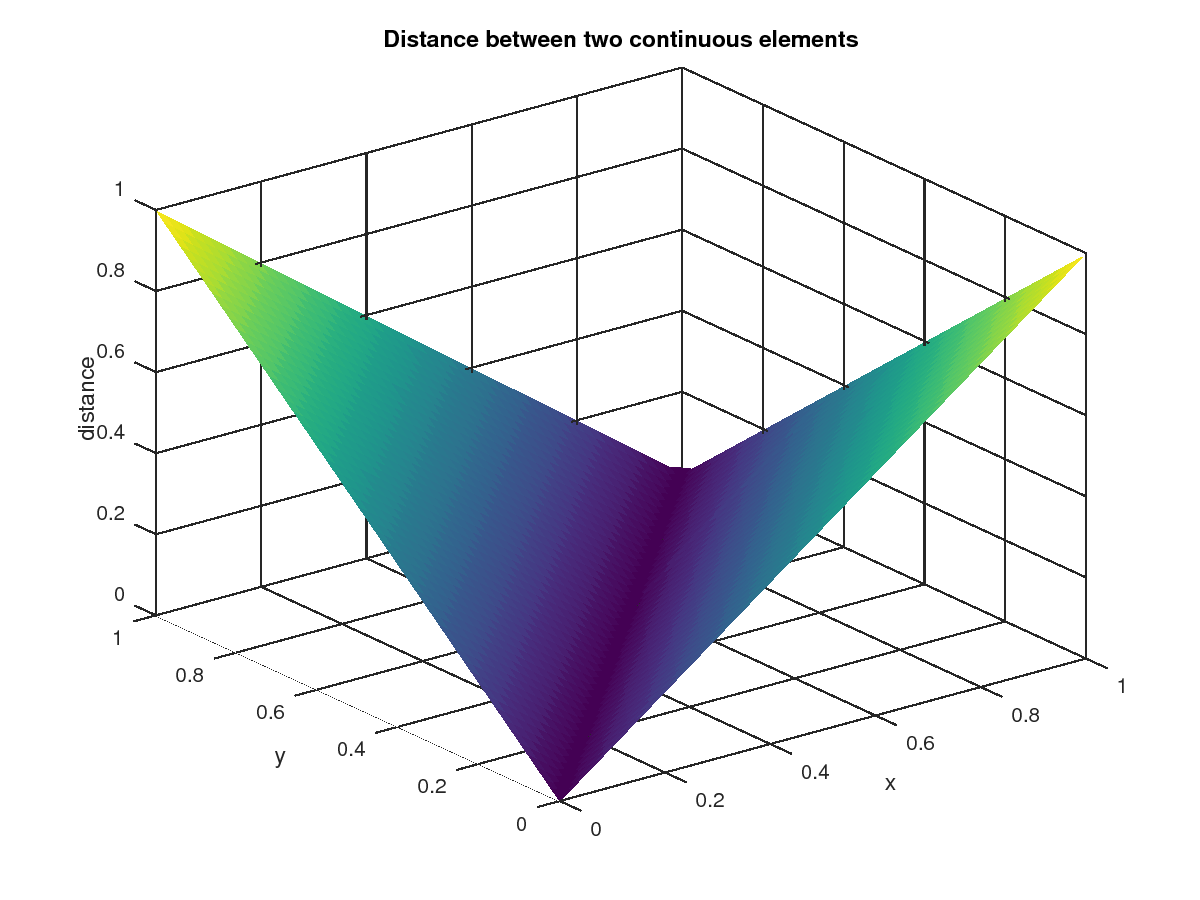
\includegraphics[width=\textwidth]{img/continuous_hamming_distance.png}
	\caption{Surface of the distance function between two continuous elements.}
	\label{fig:continuous_hamming_distance}
\end{figure*}

\subsubsection{Dataset}
The learning is based on a training data set of labeled pairs $(x_i, x'_i, s_i)$ where $x_i$ and $x'_i$ are $p$-dimensional centered training points and $s_i$ is a similarity label, whose value is 1 if $x_i$ and $x'_i$ are similar and 0 if dissimilar. To preserve a specific metric, one can compute the similarity label by thresholding the pairwise distance. Alternatively, to preserve the semantic similarity, one can assign a similarity label based on the class label. It is important to note that, if we want an exhaustive set of pairs, the number of pairs grows quadratically with the number of input vectors. With $n$ images, there are $\frac{n(n-1)}{2}$ pairs (2-combination) of input vectors.

\[D \equiv \{x_i, x'_i, s_i\}_{i=1}^N \text{ with } x_i, x'_i \in \mathbb{R}^{p} ; s_i \in \{0, 1\} \]

\subsubsection{Preprocessing}
In our implementation, it is possible to preprocess input vectors before training. Available preprocessing steps are: PCA, mean-centering and normalization to unit length, always executed in this order. Usually, only mean-centering and normalization are activated. PCA is simply implemented for experiments, to evaluate the impact of decorrelation and dimensionality reduction before hashing.

\subsubsection{Loss function}
To optimize the values of the parameters of the hash function, we define a cost function that is minimal when similarity is preserved. The cost function is inspired from Minimal Loss Hashing \cite{norouzi2011minimal}. For each pair of input vectors in the training data set, a loss function $l_{pair}: [0, 1]^{q}\times[0, 1]^{q}\times\{0, 1\}\mapsto\mathbb{R}^{+}$ assesses the quality of the mapping by assigning a cost to a pair of continuous codes and a similarity label. The cost function penalizes similar (resp. dissimilar) samples that are mapped onto continuous codes that are dissimilar (resp. similar). By minimizing the loss over all training examples, we can learn the best parameters of the hash function.

We introduce the hyperparameter $\rho$, which is a threshold of distance in Hamming space, that defines the boundary between similar and dissimilar codes. If the distance between two codes is less than (resp. more than) $\rho$ we can consider them as similar (resp. dissimilar). Although it is a slow process, a good value for this hyper parameter can be found with a validation set.

In addition, the $\lambda$ parameter adjusts the penalty incurred for dissimilar pairs when they are too close in comparison to the penalty incurred for similar pairs when they are too far from each other. In the case that there are significantly less pairs of similar images than pairs of dissimilar images, the optimization method can find a solution where all codes are different because it satisfies the majority of constraints. To mitigate this effect, $\lambda$ is equal to the number of similar pairs divided by the number of dissimilar pairs.

\[\lambda = \frac{\sum\limits_{i=1}^N s_i}{N - \sum\limits_{i=1}^N s_i}\]

Let $\norm{c - c'}_{C}$ be the continuous Hamming distance between continuous codes $c$ and $c'$. The pairwise loss based on the hinge function is defined as:

\[
	l_{pair}(c, c', s)=
	\begin{cases}
	\max(\norm{c - c'}_{C} - \rho, 0) & \text{for } s=1 \\
	\lambda\max(\rho - \norm{c - c'}_{C} + 1, 0) & \text{for } s=0
	\end{cases}
\]

\[
\begin{split}
L_{continuous}(W) & = \sum\limits_{i=1}^N l_{pair}(c_{k;W}(x_i), c_{k;W}(x'_i), s_i) \\
                  & = \sum\limits_{i=1}^N s_i\max(0, \norm{c_i - c'_i}_{C} - \rho) + (1-s_i)\lambda\max(0, \rho - \norm{c_i - c'_i}_{C} + 1)
\end{split}
\]

It is possible to find local optima where some elements of continuous codes are near to 0.5, which is not desirable when the codes are later thresholded. In this case the cost function is artificially better than it should be. To monitor the training without this bias, it is possible to compute the real cost function that takes binary codes instead of continuous codes. If the value of the continuous cost function is significantly less than the value of the real cost function, there might be elements that are not near to 0 or 1.

\[
\begin{split}
L_{real}(W) & = \sum\limits_{i=1}^N l_{pair}(b_{W}(x_i), b_{W}(x'_i), s_i) \\
            & = \sum\limits_{i=1}^N s_i\max(0, \norm{h_i - h'_i}_{H} - \rho) + (1-s_i)\lambda\max(0, \rho - \norm{h_i - h'_i}_{H} + 1)
\end{split}
\]

\subsubsection{Regularization}
To prevent the situation where elements of continuous codes take values near to 0.5, we add a regularization term that forces all elements of all codes to take values near to 0 or 1. The regularization function should output 0 if an element is exactly 0 or 1, and $r$ if it is 0.5. Moreover, the function should be smooth to ease the calculation of the gradient.

\begin{figure*}
	\centering
	
	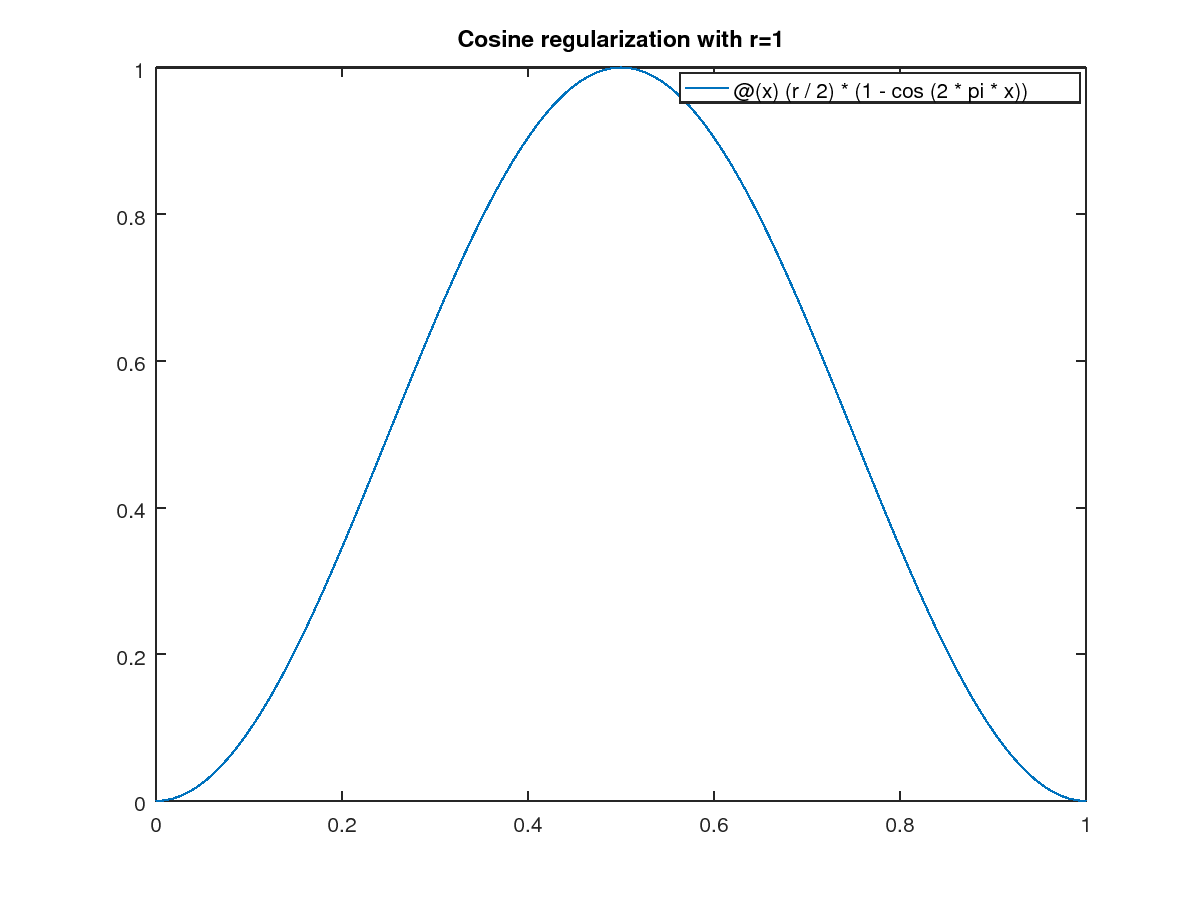
\includegraphics[totalheight=0.45\textheight]{img/cos_regul.png}
	\caption{Cosinus regularization with $r=1$}
	\label{fig:cos_regul}
	
	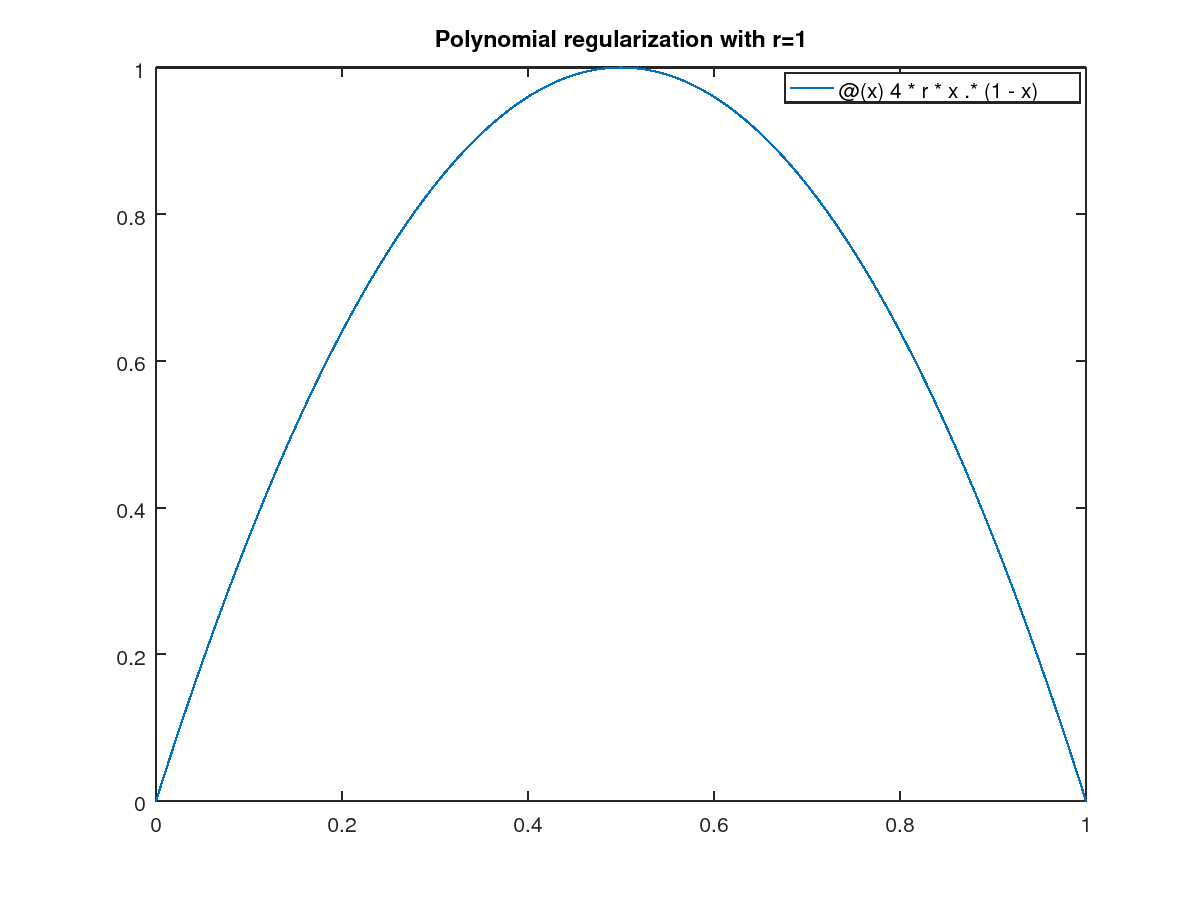
\includegraphics[totalheight=0.45\textheight]{img/poly_regul.png}
	\caption{Polynomial regularization with $r=1$}
	\label{fig:poly_regul}
\end{figure*}

\begin{figure*}
	\centering
	
	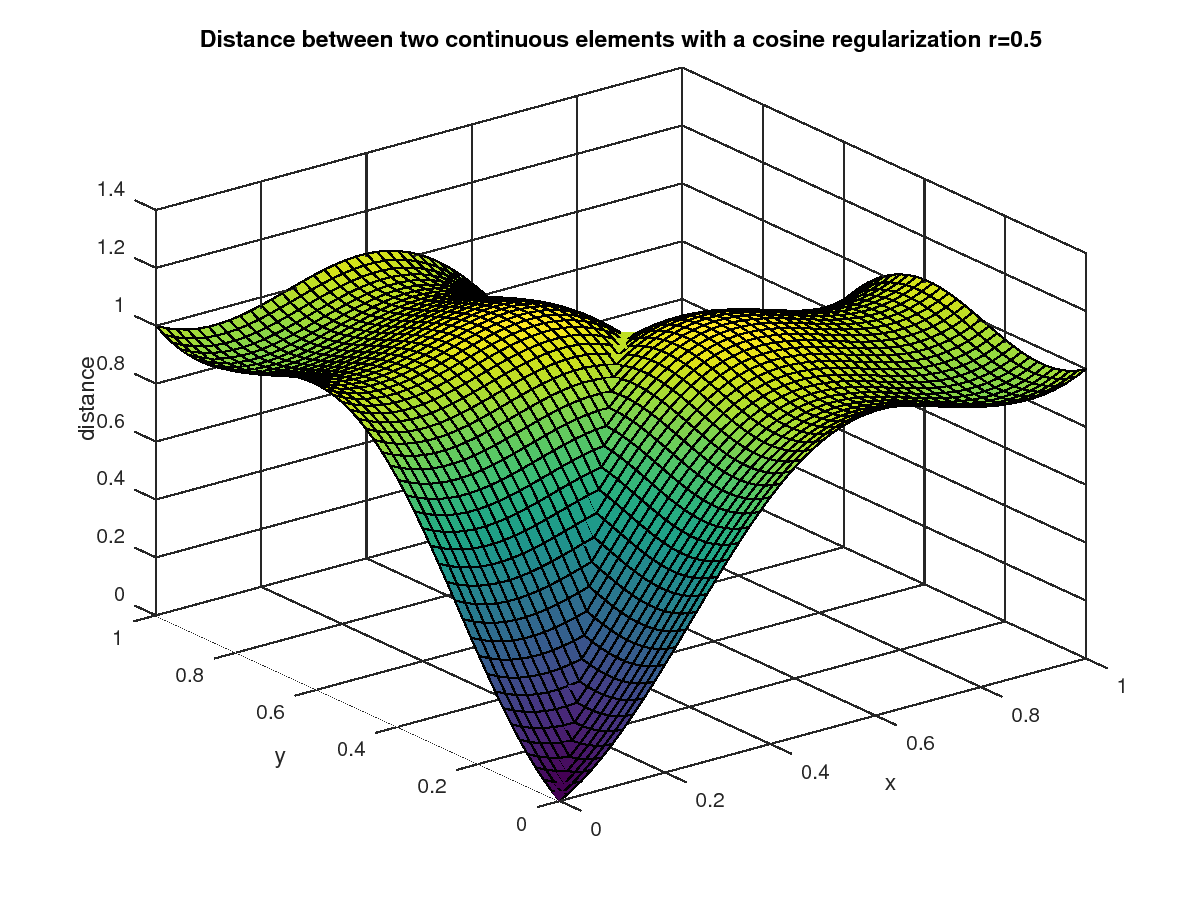
\includegraphics[totalheight=0.4\textheight]{img/distance_regul_cos.png}
	\caption{Distance between two continuous bits with a cosine regularization $r=0.5$}
	\label{fig:distance_regul_cos}
	
	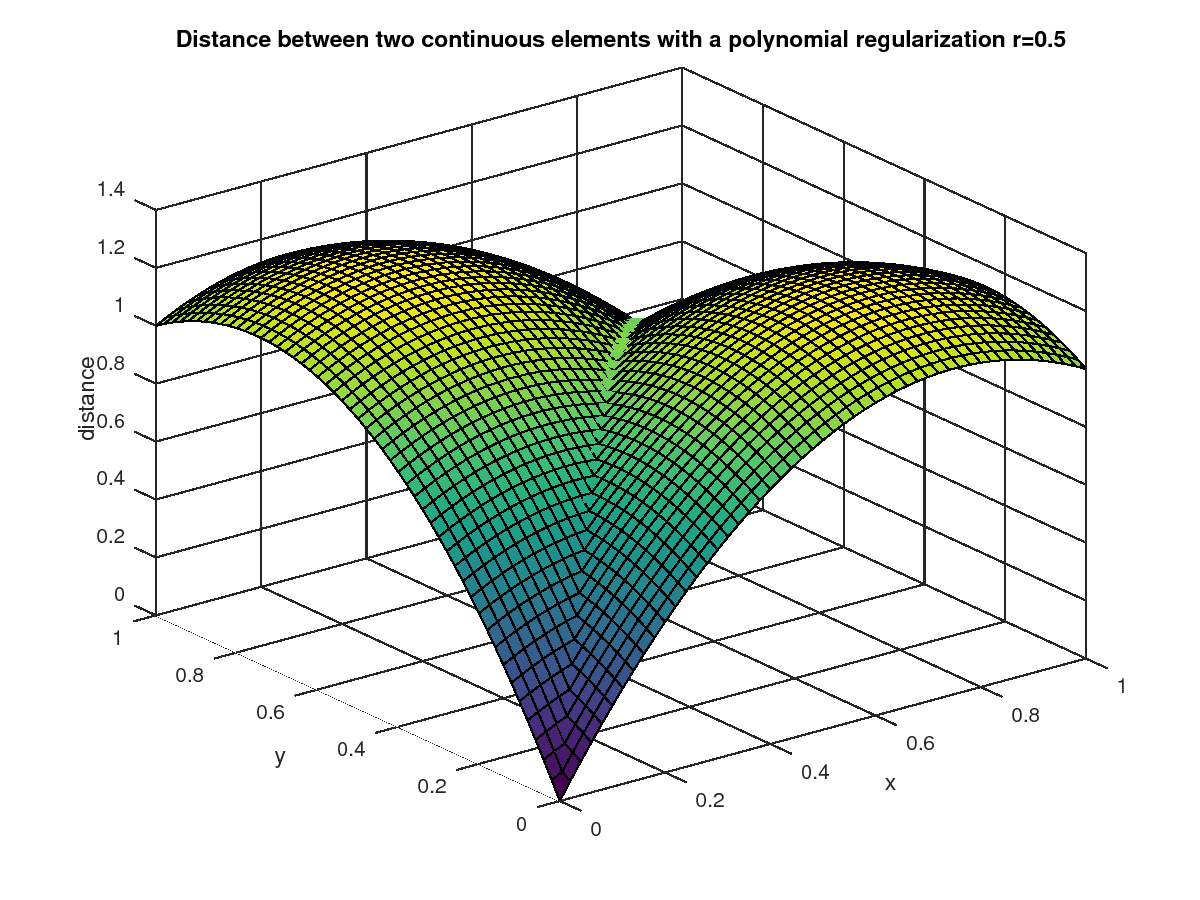
\includegraphics[totalheight=0.4\textheight]{img/distance_regul_poly.png}
	\caption{Distance between two continuous bits with a polynomial regularization $r=0.5$}
	\label{fig:distance_regul_poly}
\end{figure*}

We implemented two types of regularization: cosine (see figure \ref{fig:cos_regul}) and polynomial (see figure \ref{fig:poly_regul}). 

\[R_{cos}(x) = \frac{r}{2}(1-\cos{2\pi x}) \text{ with } r \in \mathbb{R}_{+}\]

\[R_{poly}(x) = 4rx(1-x) \text{ with } r \in \mathbb{R}_{+}\]

Cosine regularization has a null derivative near to 0 and 1 whereas polynomial regularization is steeper in these two regions.

Effect of regularization on the distance function between two continuous bits can be seen in figure \ref{fig:distance_regul_cos} and \ref{fig:distance_regul_poly}. We can see that elements near to 0.5 are penalized, therefore the distance is more than 1. The line between $(0, 0)$ and $(1, 1)$ is distinguishable from the rest of the surface, this originate from the L1 norm in the not regularized distance.

\subsection{Training}
To train the model, we compute the gradient of the cost function and use a gradient descent based method to minimize the cost.

\subsubsection{Gradient of the cost function}
To compute the gradient of the cost function, we first compute the Jacobian of $c_{k;W}(x)$, the sigmoid function.

\[c_{k;W}(x) = sigmoid_k(Wx) = \frac{1}{1 + e^{-kWx}} \text{ with } k \in \mathbb{R}_+\]

As a remainder, the $j$th element of the $i$th input vector is: $c_{k;W}(x_i)_j$. To simplify we note: $c_i = c_{k;W}(x_i)$, $c_{ij} = c_{k;W}(x_i)_j$, $c'_i = c_{k;W}(x'_i)$, $c'_{ij} = c_{k;W}(x'_i)_j$.

\[\frac{\partial c_{k;W}(x)_i}{\partial W_{ij}} = k \times c_{k;W}(x)_i(1 - c_{k;W}(x)_i)x_j\]

We then compute the gradient of the distance with the absolute value function.

\[\norm{c - c'}_{C} = \sum\limits_{i=1}^q \left|c_i-c'_i\right| \text{ with } c, c' \in [0, 1]^{q}\]

\[\frac{\partial \left|c-c'\right|}{\partial W_{ij}} = sgn(c-c')(\frac{\partial c}{\partial W_{ij}} - \frac{\partial c'}{\partial W_{ij}})\]

\[\frac{\partial \norm{c - c'}_{C}}{\partial W_{ij}} = \sum\limits_{i=1}^q sgn(c_i-c'_i)(\frac{\partial c_i}{\partial W_{ij}} - \frac{\partial c'_i}{\partial W_{ij}})\]

We then compute the gradient of the hinge functions.

\[
	\begin{split}
		\frac{\partial max(0, f(W) - \rho)}{\partial W_{ij}} & =
		\begin{cases}
		0                                     & \text{if } f(W) \leq \rho \\
		\frac{\partial f(W)}{\partial W_{ij}} & \text{if } f(W) > \rho
		\end{cases} \\[3ex]
		& = \mathbbm{1}_{f(W) > \rho} \frac{\partial f(W)}{\partial W_{ij}}
	\end{split}
\]

\[
	\begin{split}
		\frac{\partial max(0, \rho - f(W) + 1)}{\partial W_{ij}} & =
		\begin{cases}
		0                                      & \text{if } f(W) \geq \rho + 1 \\
		-\frac{\partial f(W)}{\partial W_{ij}} & \text{if } f(W) < \rho + 1
		\end{cases} \\[3ex]
		& = \mathbbm{1}_{f(W) < \rho + 1} \frac{\partial f(W)}{\partial W_{ij}}
	\end{split}
\]

Finally the gradient of the cost function is:

\[
	L_{continuous}(W) = \sum\limits_{t=1}^N s_t\max(0, \norm{c_t - c'_t}_{C} - \rho) + (1-s_t)\lambda\max(0, \rho - \norm{c_t - c'_t}_{C} + 1)
\]

\[
\begin{split}
	\frac{\partial L_{continuous}(W)}{\partial W_{ij}} = \sum\limits_{t=1}^N & s_t \mathbbm{1}_{\norm{c_t - c'_t}_{C} > \rho} \times sgn(c_{tj} - c'_{tj}) k \left(c_{tj} (1 - c_{tj}) x_{ti} - c'_{tj} (1 - c'_{tj}) x'_{ti} \right) \\
& - (1 - s_t) \lambda \mathbbm{1}_{\norm{c_t - c'_t}_{C} < \rho + 1} \times sgn(c_{tj} - c'_{tj}) k \left(c_{tj} (1 - c_{tj}) x_{ti} - c'_{tj} (1 - c'_{tj}) x'_{ti} \right)
\end{split}
\]

\[
\begin{split}
	\frac{\partial L_{continuous}(W)}{\partial W_{ij}} = \sum\limits_{t=1}^N & \left(s_t \mathbbm{1}_{\norm{c_t - c'_t}_{C} > \rho} - (1 - s_t) \lambda \mathbbm{1}_{\norm{c_t - c'_t}_{C} < \rho + 1}\right) \\
& \times sgn(c_{tj} - c'_{tj}) k \left(c_{tj} (1 - c_{tj}) x_{ti} - c'_{tj} (1 - c'_{tj}) x'_{ti} \right)
\end{split}
\]

The octave code to compute the cost function is in appendix \ref{chapter:OctaveImplementation}. 

\subsubsection{Gradient of the regularization term}
Gradient of the cosine regularization
\[
	R_{cos}(W) = \sum\limits_{i=1}^N \sum\limits_{j=1}^q \frac{r}{2}(1 - \cos(2 \pi c_{ij})) + \frac{r}{2}(1 - \cos(2 \pi c'_{ij}))
\]

\[
\begin{split}
	\frac{\partial R_{cos}(W)}{\partial W_{ij}} = \sum\limits_{t=1}^N &   \pi kr \sin(2 \pi c_{tj}) c_{tj} (1 - c_{tj}) x_{ti} \\
	                                                                  & + \pi kr \sin(2 \pi c'_{tj}) c'_{tj} (1 - c'_{tj}) x'_{ti}
\end{split}
\]

Gradient of the polynomial regularization
\[
	R_{poly}(W) = \sum\limits_{i=1}^N \sum\limits_{j=1}^q 4r c_{ij}(1 - c_{ij}) + 4r c'_{ij}(1 - c'_{ij})
\]

\[
\begin{split}
	\frac{\partial R_{poly}(W)}{\partial W_{ij}} = \sum\limits_{t=1}^N &   4rk (1-2c_{tj}) c_{tj} (1 - c_{tj}) x_{ti}    \\
	                                                                   & + 4rk (1-2c'_{tj}) c'_{tj} (1 - c'_{tj}) x'_{ti}
\end{split}
\]

\subsubsection{Optimization}
The parameters $W$ are initialized using LSH. The elements of $W$ are sampled from a normal density $\mathcal{N}(0, 1)$ and each row is normalized. Our implementation \footnote{https://github.com/mgaillard/PerceptualHashingLearning} use the fminunc function of Octave. It is possible to run the optimization multiple times with different initializations in order to take the best solution. For reproducibility, it is possible to fix the seed before the optimization. Thus, one can run the optimization multiple times with the same initialization.

To monitor the training, the continuous and real costs are displayed before and after gradient descent. If the continuous cost doesn't decrease too much, it is probably because the cost function is too hard to optimize. In this case a decreasing in the value of $k$ could help because it makes the surface of the cost function smoother. After training, a histogram of values of elements in continuous codes is computed. Ideally this histogram would contain an equal amount of values near to 0 or 1. If elements take values between 0 and 1, one could increase the value of $k$ in order to sharpen the sigmoid function, another solution would be to increase the value of $r$ in order to regularize the cost function. However, a too high value for the regularization increases the number of local minima and the cost function becomes harder to minimize. Finally, precision, recall and F-measure are computed on all pairs of images with similarity labels. If the distance between the binary codes of a pair of similar images is less (resp. greater) than $\rho$, it is a true (resp. false) positive. If the distance between the binary codes of a pair of dissimilar images is greater (resp. less) than $\rho$, it is a true (resp. false) negative. There is an example of report generated to monitor the training in appendix \ref{chapter:TrainingReport}.

% ---------------- Section: Experiments ----------------
\section{Experiments}
Experiments are conducted on the Octave implementation.

\subsection{2D points dataset}
As a first experiment, we use a dataset of random 2D points. Indeed, with only 2 dimensions, the points are very easy to visualize. Moreover, in this case hyperplanes are lines parametrized by only two values. It means that if we hash 2D points with only one bit it is possible to plot the surface of the corresponding cost function. This experiment is thus only useful to develop and visually control that our method performs well.

The input dataset is composed of $n$ clouds of $k$ points in 2D. Each cloud of point is centered around a point, whose coordinates are randomly chosen from a uniform distribution between -10 and 10. In other words, clouds are in a square of side 20 centered around the origin. To generate points in clouds, we choose each coordinate from a normal distribution of variance $s$ and whose mean is the center of the cloud. Then we generate an exhaustive list of pairs of points with similarity labels. Similar (resp. dissimilar) points come from the same (resp. different) cloud.

\subsubsection{With two clouds}
The result of our method can be seen in figure \ref{fig:hyper_2d_one_hyperplane_scatter} and the surface of the cost function is in figure \ref{fig:hyper_2d_one_hyperplane_cost}. In this example, we can clearly see that the solution is perfect. No regularization were used, $k=1$ and $\rho=0$, which means that no hyperplane should pass through a cloud.

\begin{figure*}
	\centering
	
	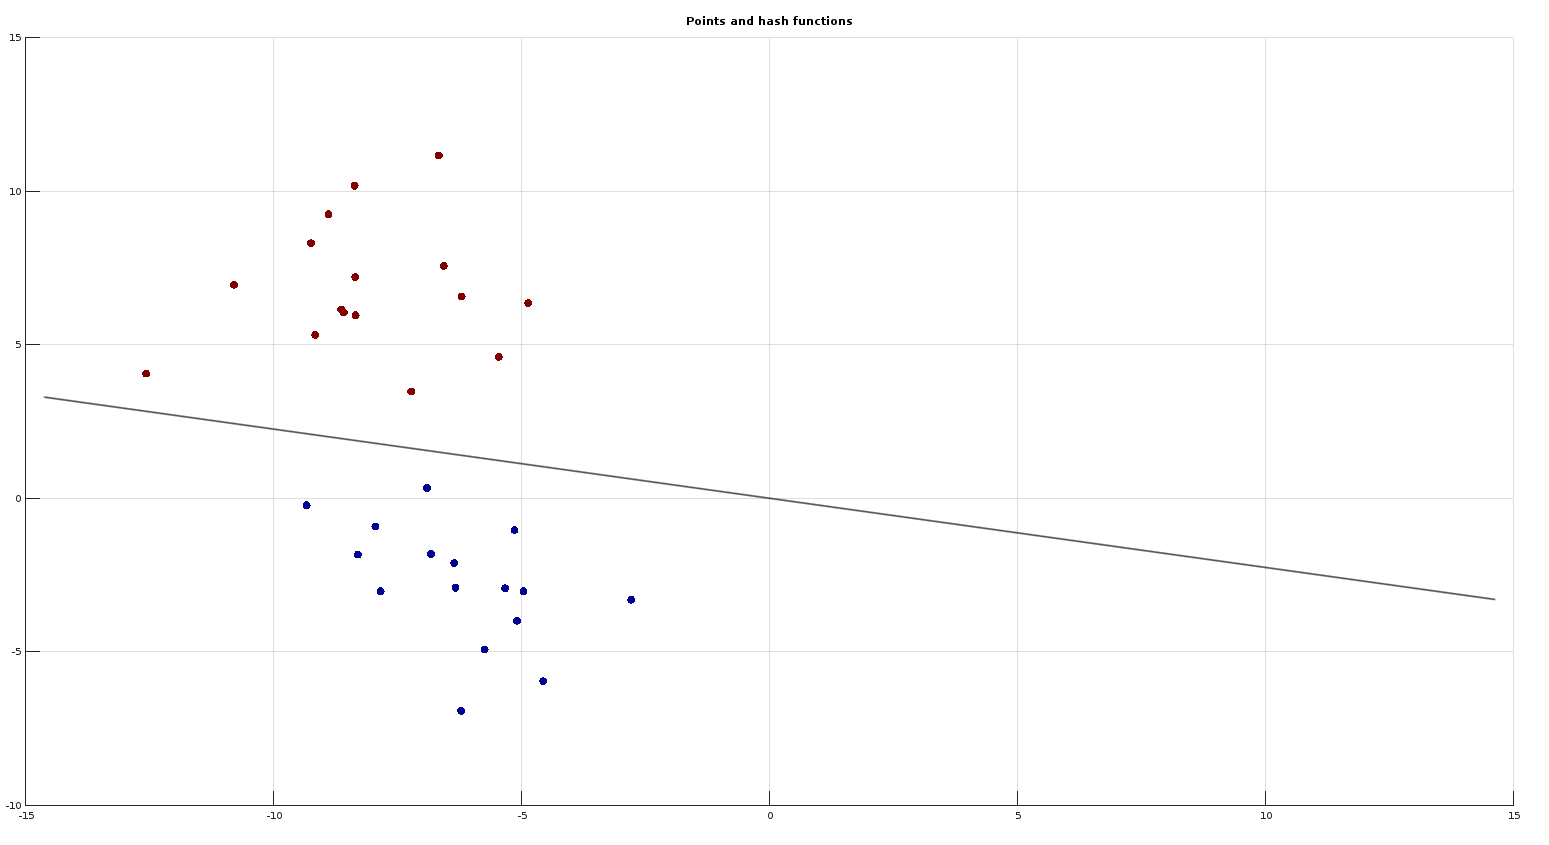
\includegraphics[width=\textwidth]{img/hyper_2d_one_hyperplane_scatter.png}
	\caption{Scatter plot of the dataset with 2 clouds of 16 points. The best hyperplane found is the black line passing through the origin.}
	\label{fig:hyper_2d_one_hyperplane_scatter}
	
	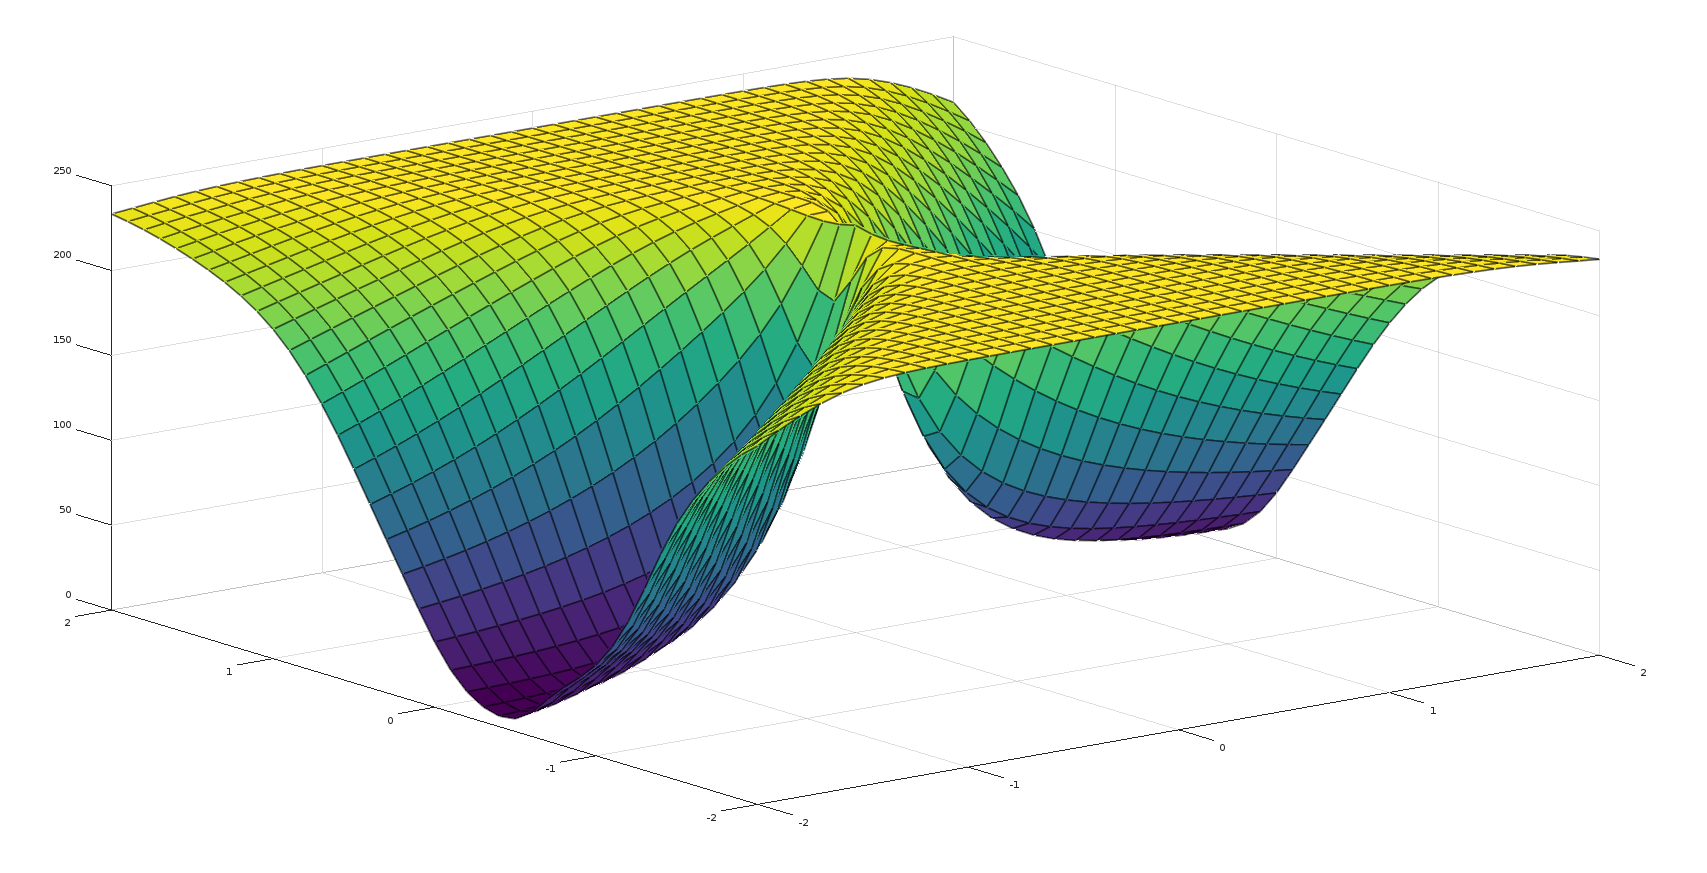
\includegraphics[width=\textwidth]{img/hyper_2d_one_hyperplane_cost.png}
	\caption{Surface of the cost function for one hyperplane in 2 dimensions and a distribution of points shown in figure \ref{fig:hyper_2d_one_hyperplane_scatter}. In this case two regions seem to be optimum.}
	\label{fig:hyper_2d_one_hyperplane_cost}
\end{figure*}

This problem is similar to the linearly separable case of SVM. There is not a maximum margin constraint but the hyperplanes are not too close to the clouds. This is probably due to the fact that the minimization in continuous space has a similar effect. Indeed, the continuous representation is never exactly equal to 0 or 1. Therefore, the optimization will force the continuous representation to take a value nearer to 0 or 1 even if the value is already near to 0 or 1. In other words, the hyperplane will stay away from the points, maximizing the margin between the hyperplane and points.

\subsubsection{With four clouds}
The result of two optimizations on 4 clouds of 16 points can be seen in figures \ref{fig:hyper_2d_three_hyperplane_scatter_easy} and \ref{fig:hyper_2d_three_hyperplane_scatter_hard}. No regularization were used, $k=1$ and $\rho=0$. The first figure \ref{fig:hyper_2d_three_hyperplane_scatter_easy} shows a case where the solution is perfect. In this particular case, only two hyperplanes would have been enough. The second figure \ref{fig:hyper_2d_three_hyperplane_scatter_hard} shows a case where a local optimum is found. One hyperplane passes through the yellow cloud. This is possible because, from the point of view of the cost function, a value of 0.5 for two similar points is considered as satisfying because no regularization is applied. 

\begin{figure*}
	\centering
	
	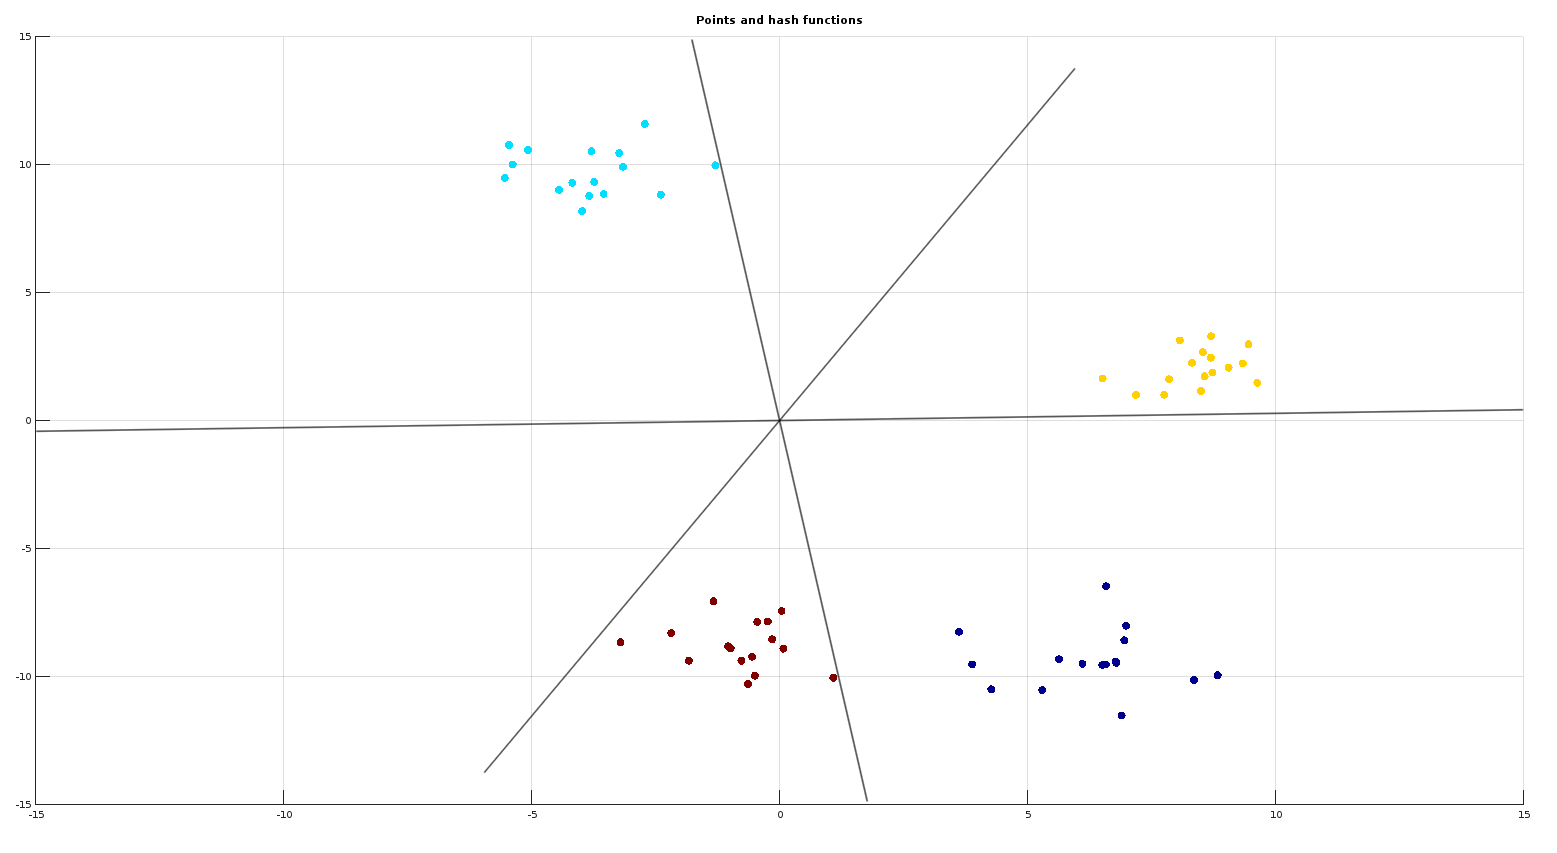
\includegraphics[width=\textwidth]{img/hyper_2d_three_hyperplane_scatter_easy.png}
	\caption{Scatter plot of the dataset with 4 clouds of 16 points. The best hyperplanes found are the black lines passing through the origin.}
	\label{fig:hyper_2d_three_hyperplane_scatter_easy}
	
	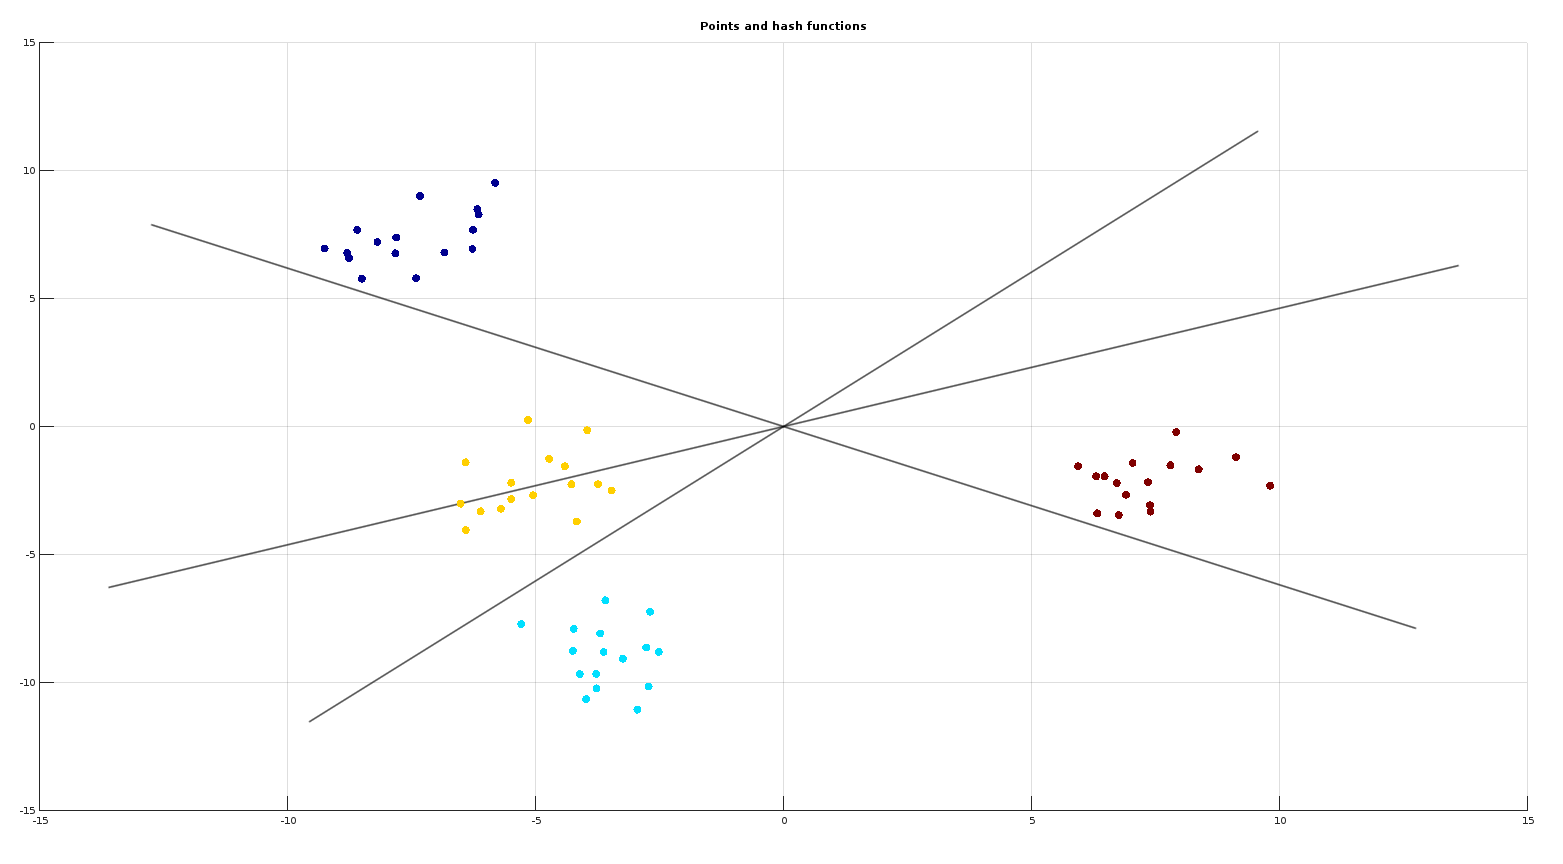
\includegraphics[width=\textwidth]{img/hyper_2d_three_hyperplane_scatter_hard.png}
	\caption{Scatter plot of the dataset with 4 clouds of 16 points. The best hyperplanes found are the black lines passing through the origin. Here one hyperplane passes through a cloud.}
	\label{fig:hyper_2d_three_hyperplane_scatter_hard}
\end{figure*}

\subsection{CNN Features dataset}
We extract features with \textit{VGG16\_block5\_pool\_max} because it has at the same time good retrieval performances and a low number of dimensions. It is desirable because the computation of the cost function is easier when features have less dimensions. 

To evaluate the quality of the hashing, we use an adaptation of our benchmark, in chapter \ref{chapter:Benchmarking}. We use the $n$ first images of MIRFLICKR \footnote{http://press.liacs.nl/mirflickr/} and their $K=6$ modified versions according to the modifications listed in section \ref{chapter:Benchmarking:section:Protocol}: blur, grayscale, resize, JPEG compression, rotation and cropping. So we have $N=(K+1)n$ images in total. The input dataset is composed of all $N(N-1)/2$ pairs of images along with their similarity labels. A pair of images that both come from the same base image is considered as similar. In the same way, a pair of images that don't come from the same base image is considered as dissimilar. So there are $n*(K+1)K/2$ similar pairs and $N(N-k-1)/2$ dissimilar pairs. Because there is too many dissimilar pairs in comparison to similar pairs, we adapt lambda so that $\lambda=K/(N-K-1)$. CNN Features are mean-centered (all at the same time) and then normalized to unit length in L2. Once training is finished, we predict the binary codes of all $N$ images and run the benchmark on the codes. It is important to note that there is no validation and test set. We learn our hash function from the actual data, thus overfitting is not a problem. Finally, we compare the precision, recall and F-measure of generated binary codes in Hamming distance to raw features with cosine distance.

Ideally, binary codes would have the same retrieval performance as raw features. It is even possible that binary codes perform better than raw features. Indeed, similarity labels stem from classes of images and not from the cosine distance between their representations. Therefore, even if angular distance is not perfect to compare image representations, it is possible to find a partitioning of the space that leads to perfect binary codes. In this particular case, the hash function learns to correct the mistakes of the image representations. This approach would be also applicable to learn the semantic similarity in a classification task. In this case, a nearest neighbor classifier would be used on the learnt binary codes.

\subsubsection{Comparison with LSH}
In this section, we compare the performances of our method to random projection. In theory, our method should perform at least as well as LSH with random projection because it is initialized exactly like LSH. We take the best model over 20 iterations for our method, and the best model over 1000 iterations for LSH. In both cases the seed is initialized with the same value. We hash the $n=50$ first images of MIRFLICKR and their modified versions (so $N=350$) on 16-bits binary codes with $\rho=3$, $k=1$ and no regularization. We plot the histogram of real cost for both methods.

\begin{table}
	\centering
	\caption{Comparison of retrieval performances of our method against LSH with random projection}
	\label{table:lsh_vs_hyper}
	\begin{tabular}{|lrrrrr|}
	\hline
	Method     & Real cost & Radius & Precision & Recall & Fmeasure \\
	\hline                          
	LSH        &       797 &  0,18 &      0,75 &   0,51 &     0,56 \\
	Our method &      21.7 &  0,18 &      0,99 &   0,92 &     0,95 \\
	\hline
	\end{tabular}
\end{table}

\begin{figure}
	\centering
	
	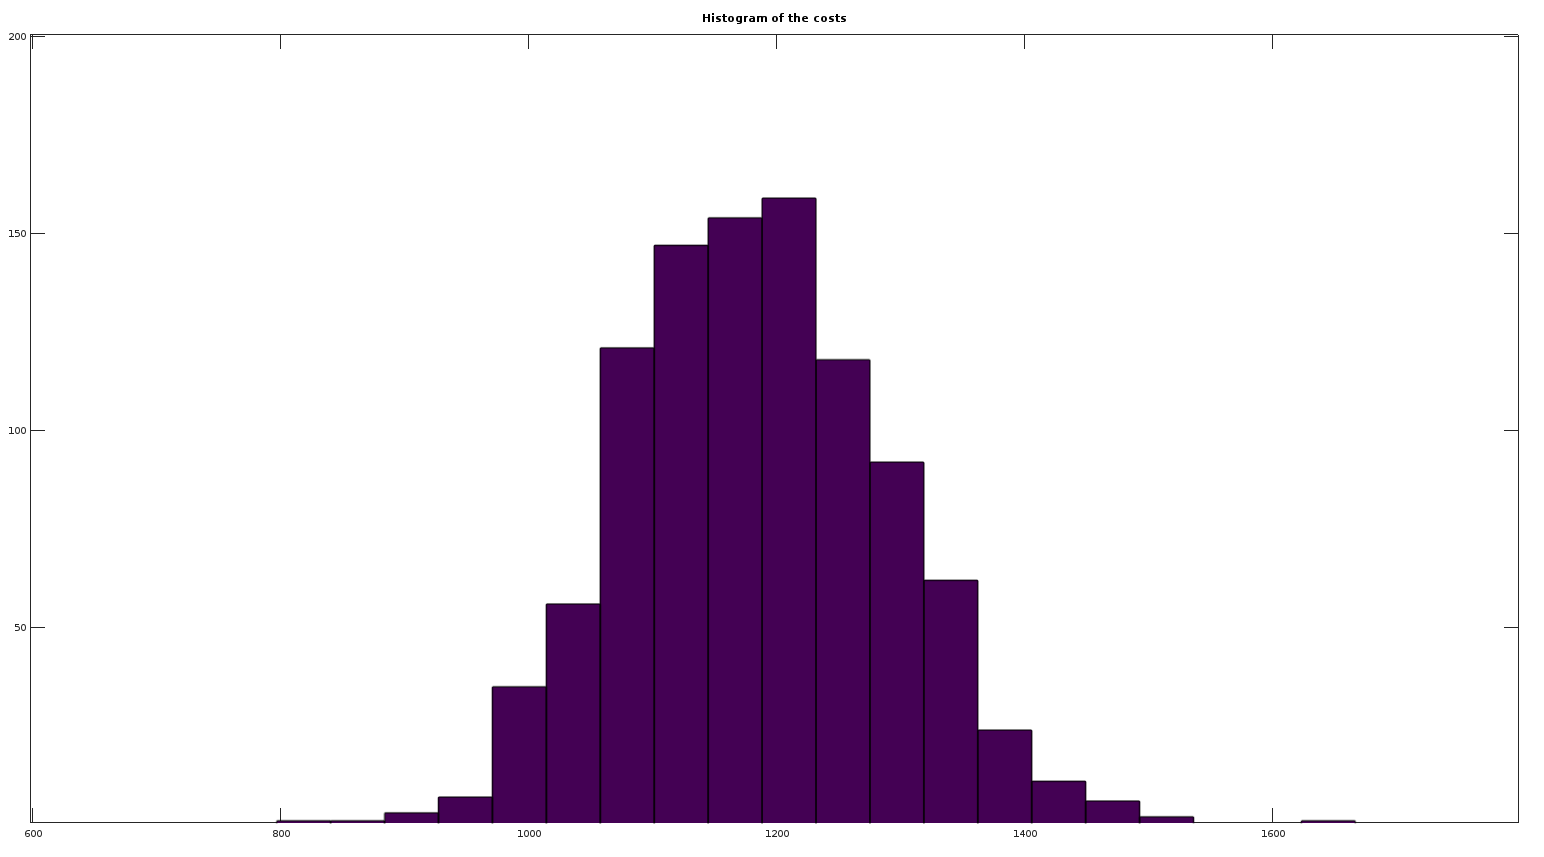
\includegraphics[width=\textwidth]{img/lsh_best_of_1000.png}
	\caption{Histogram of real cost for 1000 iterations of LSH.}
	\label{fig:lsh_vs_hyper_best_of_1000}
\end{figure}

Results are in table \ref{table:lsh_vs_hyper}. The histogram of cost function for LSH is shown in figure \ref{fig:lsh_vs_hyper_best_of_1000}, the mean cost is 1184 and the standard deviation is 106. With 1000 iterations, we can say that LSH is not likely to produce solutions that are really better than the one that we found with the minimal cost of 797. So the F-measure of 0,56 obtained with LSH is a upper bound of the performance of LSH. Our method achieves every time a better solution than LSH with a maximum real cost of 81. The mean real cost is 37.8, the standard deviation is 14.8 and the minimum real cost is 21.7. We can see that our method achieves every time a higher F-measure than LSH with random projection. By the way, it is interesting to note that the best F-measure is reached with a radius of 0.18, which is approximately equal to $\rho / 16$.

% ---------------- Section: Conclusion ----------------
\section{Conclusion}
In this chapter, we present a new approach to learn a hash function for CNN Features. Although our experiments are superficial and can't prove that our method yields state of the art performances, we have very promising results. With more time, we could have conducted more experiments. Some questions are still open: what is the influence of the regularization? How well our method performs when the number of bits increases, when the number of images increases?

The effect of regularization on the distance between two continuous elements could be better. Cosine regularization seems to introduce local minima in the cost function, thus the solutions are often worse with regularization. We didn't extensively test the polynomial regularization, but this one seems to introduce less local minima than cosine regularization. For the moment by choosing the right value for $k$, the regularization is not necessary, but this is a complicated process.

The $k$ parameter is redundant because rows of $W$ are unconstrained, they can take a big value, which is equivalent to a big $k$. We need to evaluate the effect of $k$ and whether it is really required. There seems to be two options, either we keep $k$ and we normalize the rows of $W$, or we remove $k$ and we don't normalize $W$. 

Because our implementation uses the fminunc function of Octave, we can't have an effect on the minimization of the cost function. What we could do is to plot the real cost along with the continuous cost during learning, in order to monitor the optimization. We could also change the pairs of images in the dataset during the training to select at each step only the pairs that bring the more information.

During the training, we select the best model over multiple iterations by choosing the one with the minimum real cost. However, it is not proven that selecting the lowest real cost is equivalent to selecting the highest F-measure. 

The optimization is not easy, the algorithm often falls into a local optimum and to find a satisfying optimum we need to rerun several times the gradient descent with various random inputs. Is it possible to use another optimization method that is less prone to falling in local minima? If we add hidden layers before the hashing layer, shall it be easier to optimize? In facts, the hidden layers can change the input space to ease the training of the last layer. At the end, the objective would be to program a loss layer with a neural network framework. This would allow us to use it on top of a neural network and learn non-linear projections. Moreover, we could use the GPU implementation of the framework to fasten the computation of the cost function.

Scalability is not perfect because the number of pairs of images grows quadratically. For this reason, the number of images is deliberately low because the cost function is hard to compute with a big dataset. For example, with a total of 1400 images, there is about 1 million pairs of images, which is huge. With a GPU implementation, we could go further but definitively not up to a big number of images. Another solution that we explored is to select only the pairs of images that bring the more information, because dissimilar triplets are mostly redundant. Unfortunately, we didn't have the time to evaluate extensively this option. Currently the way to apply this method to large scale reverse image search is to train the model on a small number of images with a validation set and hope that it will generalize on more images.
